\chapter{Heritage of ice reservoirs}

\cleanchapterquote{Before the artificial glacier, we struggled to get any barley. But now we can grow many
	crops, even potatoes, which need to be planted earlier in the spring, but sell for much more money.
}{Tashi Tundup}{(A 76-year-old farmer in Ladakh, India)}

Climate warming has resulted in the retreat and thinning of mountain glaciers
\citep{ipccCrossChapterPaperMountains2022}. This has implications for water availability in river basins with
considerable glacierized areas in their headwaters, such as \ac{HMA}. Glaciers in \ac{HMA} provide an important
gradual release of water that is used by many people locally and downstream for irrigation, drinking water, and
hydropower. Climate change in this densely populated region can have serious consequences for glacier meltwater
supply to the rivers \citep{immerzeelImportanceVulnerabilityWorld2020}. In this context, the development of
water storage technologies like \ac{AIRs} (Fig. \ref{fig:airs_ladakh}) is crucial to ensure continued sustenance
of cryosphere-fed irrigation networks.

\begin{figure}
	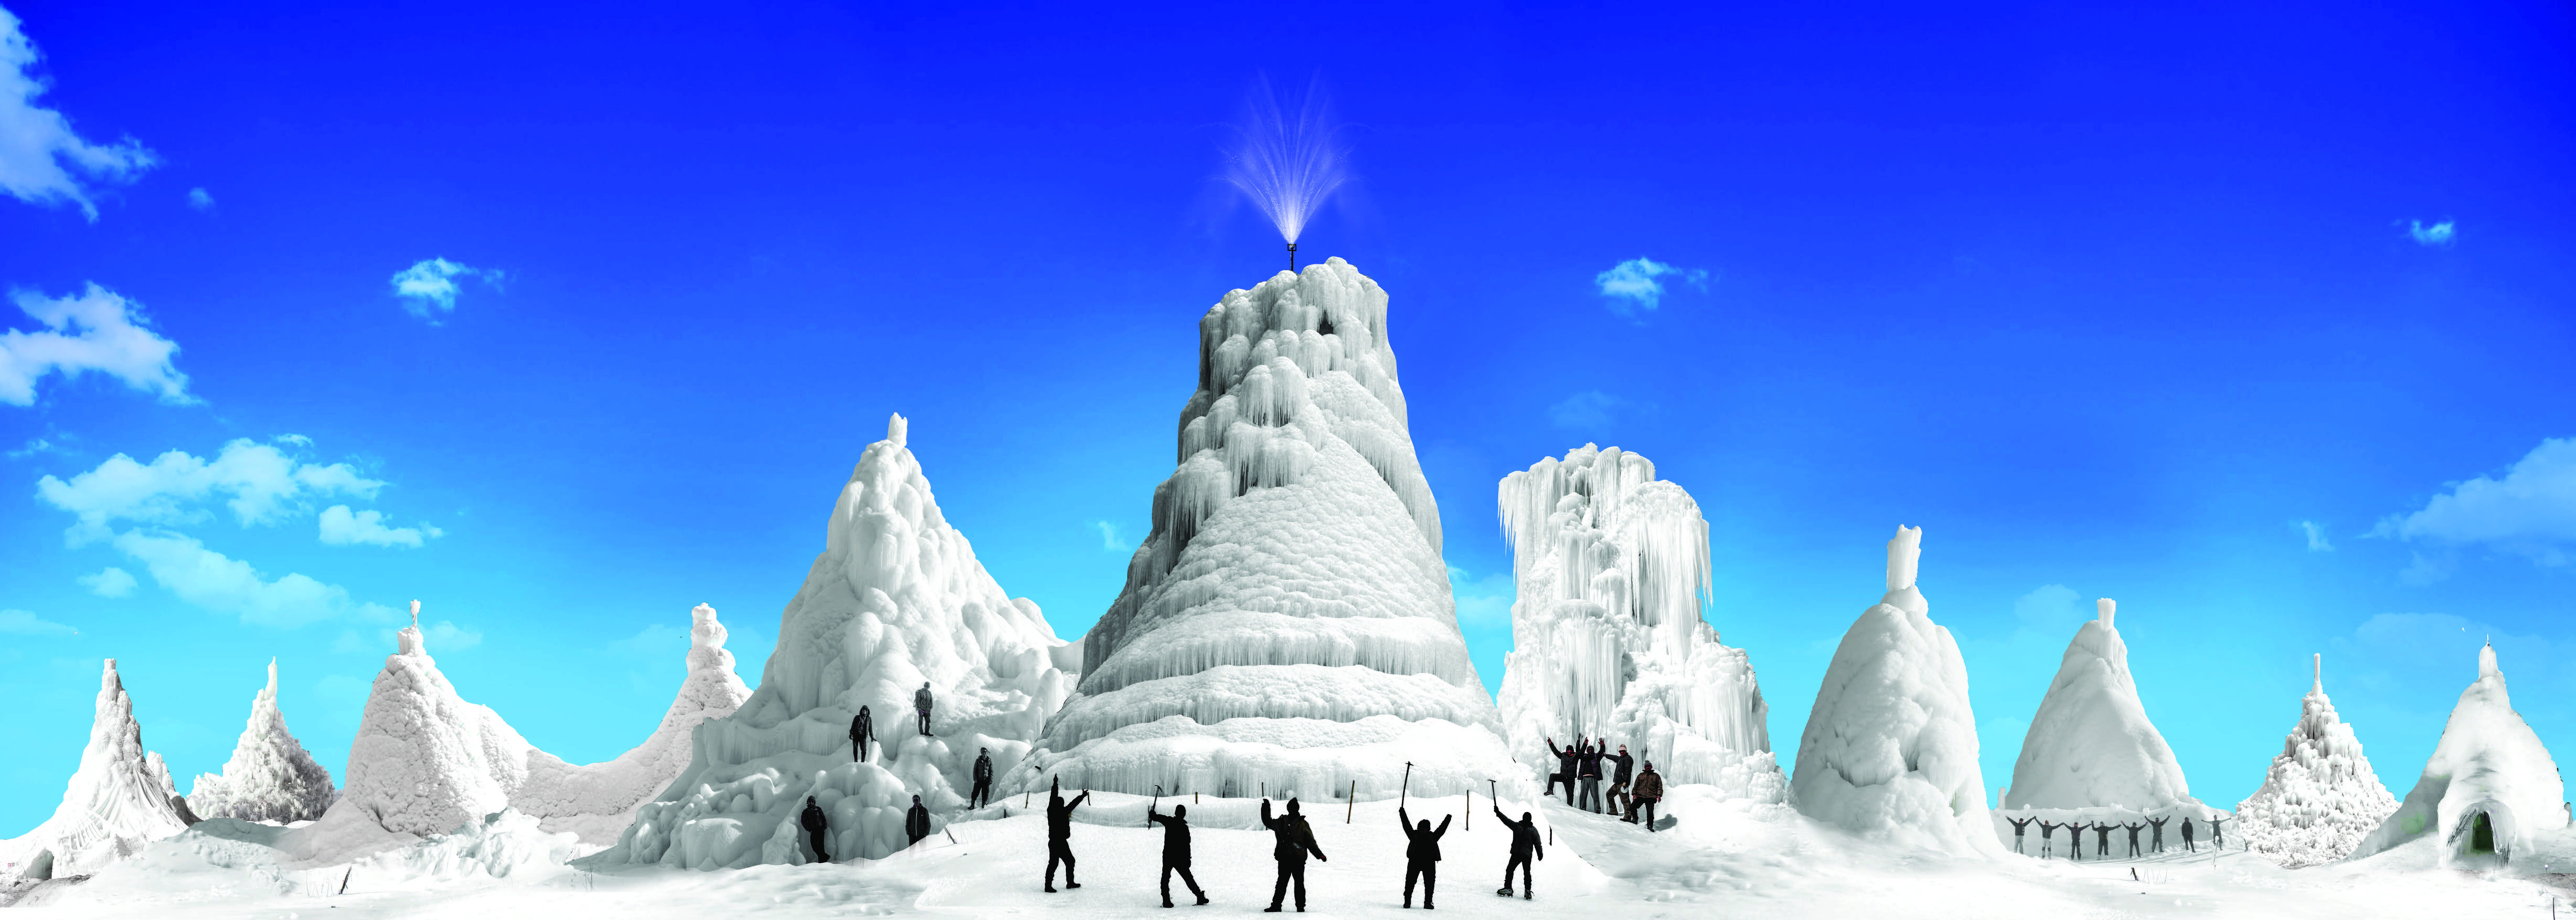
\includegraphics[width=\textwidth]{figs/AIRs_Ladakh}
	\caption{Compilation of \ac{AIRs} built in different villages in Ladakh.}
	\label{fig:airs_ladakh}
\end{figure}

The studies presented in this thesis provide insights into the volume evolution of \ac{AIRs}. However, various
research gaps still remain and need to be overcome before \ac{AIRs} can be integrated into water resource
management plans. Moreover, further development of the construction tools is required to improve the
cost-effectiveness, size, and survival duration of \ac{AIRs}. In this context, we highlight some of the
challenges and discuss possible approaches to overcome them below:

\section{Discussion and challenges}


\subsection{To improve data collection and model approaches}

Modelling is a powerful tool that allows to identify the causes of AIR volume dynamics in space and time.
Improvement of modelling approaches introduced in the \textit{Science} chapter can lead to identification of
other favorable construction regions, effortless operation of the fountain and integration of nature-based water
storage technologies in water resource management plans. Specifically, use of the COSISTUPA model is indicated
for future estimations of \ac{AIR} volume. This model needs to be extended so that it can account for future
climate variability and produce accurate meltwater predictions. Modelling the future is fundamentally different
from simulating the past: for the past, the model serves as a tool for interpreting and best exploiting field
measurements---and can be directly constrained by them; for the future, climate variability must be comprehended
to be able to yield realistic projections. Almost all methodological steps in the modelling of future \ac{AIR}
runoff are subject to potential enhancements. Model accuracy can be enhanced with the following methods:


\subsubsection{Quantity and quality of calibration and validation datasets}

The calibration and validation processes used present inherent temporal and spatial biases due to the following
subjective choices:

\begin{itemize}
  \item \textbf{Number and timing of surveys.} The number of \ac{GPR} and drone surveys need to be increased for
    better calibration and validation. Moreover, the timing between each of these surveys need to be uniformly
    distributed across the study period. For example, among the five drone surveys of the IN21 \ac{AIR}, most of them
    were conducted around early March, when the \ac{AIR} volume was near its maximum, whereas the seven drone
    surveys of the CH21 location were more evenly spaced out. This observation bias responds to logistical
    issues in conducting measurements at regular intervals.

  \item \textbf{The meteorological conditions under which surveys are performed.} In particular, precipitation
    events reduce \ac{DEMs} quality generated from drone surveys, since they create uniform snow surfaces over
    \ac{AIRs}. These surfaces do not allow the identification of features that can be used to extract the radius
    and area of the \ac{AIRs}. \ac{GPR} surveys, on the other hand, also cannot be conducted during
    precipitation events due to logistical issues. 

\end{itemize}

Thus, the quality of volume validation is limited by the uncertainties associated with conducting and analysing
the surveys. This limitation can be overcome by extending the model validation set using two approaches. First,
measuring daily \ac{AIR} meltwater quantities; accuracy of this validation method depends on the wind speeds of
the location but can be improved if the terrain is made waterproof and oriented so that most of the \ac{AIR}
runoff can be collected. Second, analyzing \ac{GPR} surveys further; \ac{GPR} is sensitive to subtle changes in
the properties of ice layers, making it a powerful tool to image the internal structure of ice structures. For
example, \ac{GPR} surveys conducted on the IN21 \ac{AIR} \citep{balasubramanian_suryanarayanan_2022_7056646} can
be further used to validate internal density variations.

\subsubsection{Albedo parametrization}

The albedo parametrization illustrated by equation \ref{eqn:alb} had to be modified to accomodate fountain
discharge events. The influence of fountain discharge events on albedo can be considered to be similar to
rainfall events. However, literature suggests that influence of rainfall on albedo variation is not
straightforward. A heavy rainfall event can lead to a short-term (between 1 and 4 days;
\citet{azzoni_estimating_2016}) increase in albedo due to decreasing surface roughness and/or wash-out of fine
debris present on the ice surface \citep{brock_analysis_2004, azzoni_estimating_2016}, whereas light rainfall
can cause the presence of a thin water film on the ice surface that absorbs radiation much stronger than the
underlying ice and thus results in a decreased albedo. Inclusion of such processes is not possible in the
framework of the \ac{AIR} model. Therefore, a simplistic approach of increasing the decay rate by a constant
factor after every fountain discharge event was chosen. However, the value of this factor has no basis on
measurements. Field-based albedo measurements are required to better parametrize the effect of water spray on
the surface albedo decay rate.

\subsubsection{Turbulent heat flux parametrization}

The method used to calculate turbulent heat fluxes by \citet{garrattAtmosphericBoundaryLayer1992} assumes that
these fluxes act over a uniform planar surface. This leads to the use of a exposure/roughness parameter
$\mu_{cone}$ as a correction factor. However, equation \ref{eqn:mu} about $\mu_{cone}$ is just an educated
guess. To base estimates of this parameter on information in literature is difficult. Many studies have been
performed on the effects of obstacles on atmospheric boundary layer flow (e.g., trees), but always in an
ensemble setting, focusing on the bulk effect of an ensemble of obstacles. In this thesis, the case is that of a
single obstacle in open terrain, and the roughness of the surface and the exposure are likely to lead to larger
turbulent fluxes.

\subsubsection{Spray radius quantification}

All models require the fountain spray radius as input. This is a significant limitation, since these models are
very sensitive to the spray radius parameter. Moreover, spray radius is not only determined by fountain
characteristics but also by wind-driven redistribution, refreezing, and melting events across the \ac{AIR}
perimeter. The same fountain was observed to produce different spray radius values corresponding to different
winters for the Swiss experiments. Further discussion on this can be found in Section \ref{sec:interannual}.

\subsubsection{Quantification and development of ice terraces}

Although this thesis focuses on ice stupas, their ice volumes pale in comparison with ice terraces
\citep{nusserSociohydrologyArtificialGlaciers2019}. This is because ice stupas are limited by their fountain's
spray radius. Ice terraces have no such limitations. Their thickness is only limited by the water supply rate or
meteorological conditions, and they can occupy any construction area provided. However, ice stupas are the
preferred method for ice harvesting since they can be constructed in relatively lower altitudes, with lesser
effort and at a lower cost.

With a suitable redesign of the automation hardware, automated construction strategies can also be applied to
ice terraces. Such a construction strategy can potentially compound their size every consecutive winter with
minimal maintenance requirements. Therefore, future research should aim to answer the following questions:

\begin{itemize}

	\item How can ice terrace construction systems be engineered to reduce water losses and maintenance
	      efforts?

\end{itemize}

The methodology developed in this thesis can also be applied in such an analysis.

\subsubsection{Adaptation potential of glacierized catchments with AIRs}

Vanishing glaciers, natural hazards (such as inundations, mudflows, and landslides), decreasing river discharge,
drying springs, next to shifts in precipitation patterns are apparent climate change impacts which affect
glacierized catchments.

In the Peruvian Andes, both water scarcity (low-flow water risk) and glacial lake outburst floods (high-flow
water risks) could have an important impact on local population, infrastructures, and economic activities
\citep{motschmannIntegratedAssessmentsWater2020}. For example, the estimated loss in annual wheat output due to
reduced glacial runoff would be to the tune of 18 million USD, even in the low emission scenario of Quillcay
catchment in Peru \citep{motschmannLossesDamagesConnected2020}. Similarly, in the Stok catchment in Ladakh,
glacial ice reserves have shrunk by more than 18\% in the past 16 years, leading to a decline in crop
productivity \citep{sohebSpatiotemporalQuantificationKey2022}.

\ac{AIRs} can already buffer from low-flow water risks in certain catchments. For example, some ice terraces in
Ladakh have been measured with areas up to 19\% of the Stok glacier (0.8 $km^2$)
\citet{nusserSociohydrologyArtificialGlaciers2019}. With further technology development, \ac{AIRs} can also be
used to mitigate high-flow water risks. The glacial lakes of the Andes and the Himalayas can be siphoned to form
\ac{AIRs} at scales that can last perpetually. Such \ac{AIRs} can compound over the years and become another
source of perennial water supply for the respective catchments.

\subsection{To improve hardware tools}

The \textit{Technology} chapter shows one strategy that can improve the water-use efficiency of \ac{AIRs}. This
strategy was chosen because it enables the use of the \ac{AIR} model in a simple and effective manner. However,
all these construction strategies are limited by the tools they use, namely the fountain and the pipeline. From
a scientific point of view, the methodology is not suitable to quantify and optimize these hardware tools. This
is discussed below, and some recommended methodologies for improvement are provided:

\subsubsection{Fountain optimization}

Contrary to the model assumptions, the parameters used to define the fountain were not independent. The fountain
height, aperture diameter, discharge rate, water temperature, and spray radius were related through the
trajectories of the water droplets. The fountain nozzle design is crucial for increasing the ice volume
obtained. It determines the diameter of the water droplets and the angle of launch for their projectile motion.
The choice of these two parameters determines the rate of the nucleation process, pressure losses, and discharge
rate ranges. For example, during the IN21 experiment, snow formation was observed, indicating the potential of
the fountain water droplets to freeze before deposition on the \ac{AIR} surface. In the CH22 experiment, the
higher aperture diameter of the nonscheduled fountain nozzle (Fig. \ref{fig:autovsman}) produced bigger droplets
and, therefore, had a lower fountain pressure loss compared with the scheduled fountain. However, fountains with
large aperture diameters lose their ability to form water droplets at low discharge rates. Therefore, the
scheduled fountain nozzle design was used, since it was able to produce water droplets with discharge rates as
low as 2 $l/min$.

However, no methodology currently exists to rank the different fountain nozzles used for construction. Quantifying
processes influenced by the fountain nozzle is challenging, as this would require the modelling of the conduction,
convection, wind redistribution, and nucleation processes that droplets of varying diameters undergo during
their flight time. Instead, controlled experiments comparing the freezing rates among different fountain
diameters have a better chance to yield insights on the engineering design of fountain nozzles.

\subsubsection{Pipeline optimization}

An ideal pipeline configuration could make this technology cheaper and maintenance free. However, optimization
of the pipeline material and diameters is yet to be performed---despite the time lost on pipeline freezing
events and the potential cost reduction with cheaper pipeline materials and sizes. Larger pipeline diameters
reduce the occurrence of pipeline freezing events but increase the cost dramatically. In Ladakh, pipeline
diameters used have a wide range (from 0.03 to 0.3 $m$), since the choice of pipeline diameter also depends on
the additional insulation provided and on whether or not it is buried. Therefore, a comprehensive cost--benefit
analysis of different combinations of insulation and pipeline materials is required to determine the optimum
design of the insulated pipeline system.

\subsubsection{Cost reduction of automation system}

The strategy presented in this thesis is not yet suitable for application in current \ac{AIR} construction sites
due to the cost of the automation system (around 8000 USD). However, an up to 10-fold cost reduction can be
possible through simpler automation systems that control only the duration of fountain spray, not their
quantity. 

\subsection{To improve site selection of AIRs }

Farmers in \ac{HMA} have been improving ice harvesting technologies for generations, as documented in the
\textit{Tradition} chapter. But these technologies can also be leveraged by farmers in many other regions. In the
absence of an objective global-scale estimation of \ac{AIR} water storage, we propose some subjective guidelines
that can help narrow down favorable construction sites.

\subsubsection{Meteorological and topographical considerations for AIR site selection}

Two sets of guidelines are proposed in this thesis to identify future construction sites at regional and local
scale. These suggestions are guided by the different case studies presented in this thesis and field experiences
in Ladakh over the past six winters.

\textbf{Regional scale}

\begin{enumerate}

	\item Minimum median monthly temperature less than $0 \degree C$ to ensure sufficient freezing rate.
	\item Water supply with median discharge rate more than $2\, l/min$ to ensure sufficient water supply.

\end{enumerate}

\textbf{Local scale}

Given a valley or a region satisfying the above requirements, further selection of sites around the particular
water supply can be performed using the criteria below:

\begin{enumerate}
	\item Higher water source temperature to minimize risk of pipeline freezing events.
	\item Terrain slope between water source and site greater than 20 $m$ every $km$ to ensure sufficient
    gravitational head for fountain operation.
	\item Low daylight hours to decrease solar-radiation-induced melt.
	\item Higher altitude for higher freezing rates.
\end{enumerate}

\subsubsection{Sociohydrological considerations for AIR site selection}

In this section, we illustrate the role of place in AIR construction by comparing the
contrasting responses of villagers to two AIRs constructed in the Phyang village of Ladakh (Fig. \ref{fig:phyang}). The first AIR site was on the main stream bed at the 
upper end of the village of Phyang; this stream has for centuries been used to irrigate the fields of Phyang and 
the village of Phey, located downstream. The other AIR site was in an arid area called the Thang, which lies 
outside the conventional watershed of the Phyang village. The Thang AIRs were
promoted as part of a desert reclamation project to irrigate a small plot of poplars and fruit trees located next
to them. However, the inhabitants of Phyang and Phey – the intended beneficiaries of the Ice stupas – remained unimpressed.
Whereas, the second AIR built next to the main stream bed, 
upstream from the village of Phey has not been contested and has been even cautiously accepted.

\begin{figure}
	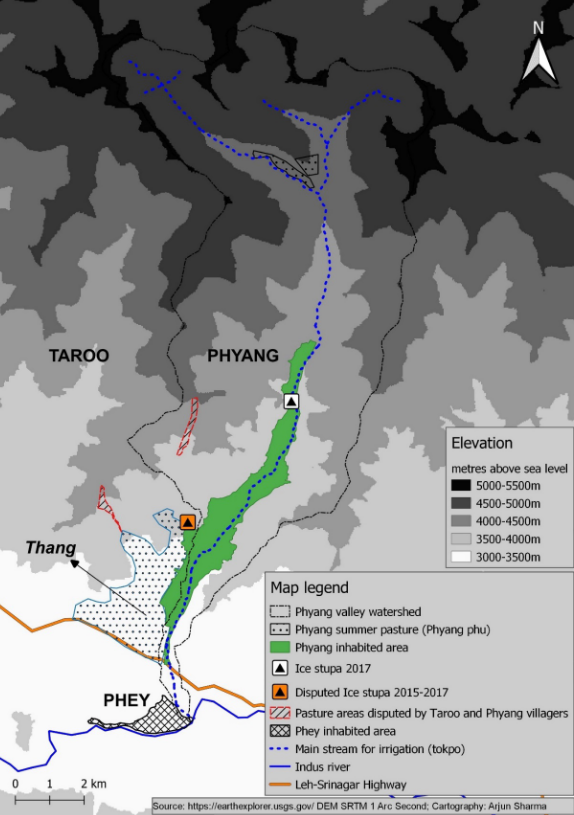
\includegraphics[width=\textwidth]{figs/sharma2019.png}

  \caption{The two AIR sites in the village of Phyang. Source: \citet{sharmaGivingWaterIts2019}}

	\label{fig:phyang}
\end{figure}

Why is it that AIRs located at different locations in the same village are received so differently by their
intended beneficiaries? \citet{sharmaGivingWaterIts2019} argues that this is because of the following two
reasons:
\begin{enumerate}
  \item While the developers of the AIRs want to use the arid construction site (the Thang) to showcase 
    their commitment to global sustainable development discourses, the villagers of Phyang want to use it 
    for commercial and residential purposes.
  \item The AIR uses a water source that is considered to be shared by two villages. As such, it is contested
    because it transgresses the original watershed boundaries covered by the present customary irrigation
    governance regime.
\end{enumerate}

\subsubsection{Socioeconomic considerations for AIR site selection}

A better understanding of how AIR construction efforts are integrated in the broader mountain development process 
requires a consideration of political power and economic exchange. In the case of Ladakh, The land use strategies are 
characterized by their efforts to improve livelihood security through flexible integration of subsistence-based agriculture
and off-farm activities \citep{nusserIrrigationDevelopmentUpper2012}. The growing number of households involved in nonagrarian
activities leads to AIRs used more as a touristic attraction rather than as a water storage device in these
communities. As a consequence, the site selection of such AIRs are optimized based on their proximity to roads
and their design is guided by artistic motivations.

% \subsubsection{New ways to upscale irrigation water supply}
\subsection{To improve operation of AIRs}

In this section, two hypothetical ice stupa construction scenarios----namely, present and future---are
described. The present scenario is a depiction of the construction efforts based on oral interviews and field
experience. The future scenario is a depiction of how the automation system developed in the \textit{Technology}
chapter can transform current construction efforts. The objective of both scenarios is to maximize the meltwater
quantity available for irrigation. Both scenarios are motivated by the construction campaigns conducted in the
Gangles valley in Ladakh during the winter of 2019/20 (Fig. \ref{fig:gangles_data}). This is the same valley
where the IN21 study site was located, enabling us to extrapolate some of the freezing rates and ice volume
estimations from paper I. Conservatively, the valley is assumed to have a total water supply of around
$120\,l/min$, a winter duration is assumed to be 4 months, and the fountain is assumed to be  operational for
only 8 h per day for both scenarios. 

\begin{figure}[htb]
	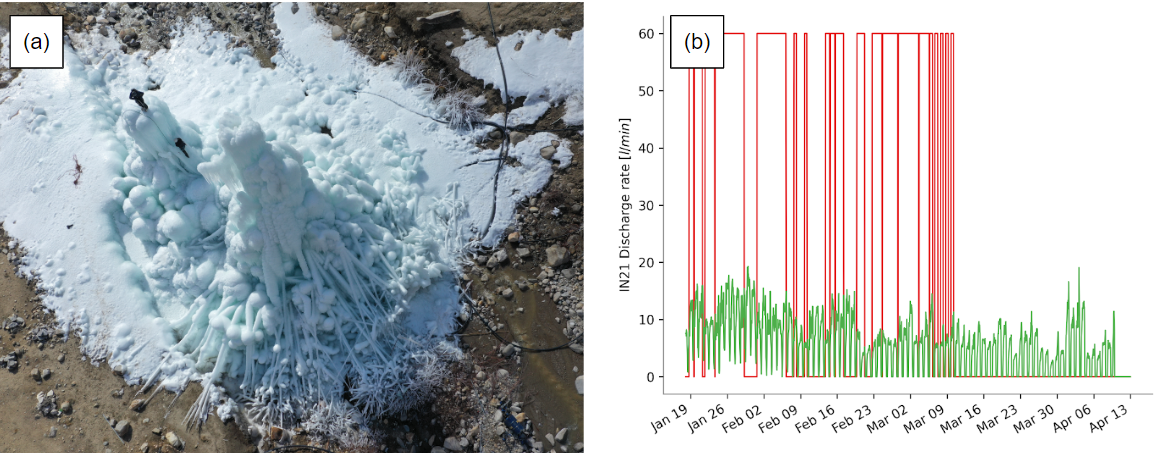
\includegraphics[width=\textwidth]{figs/gangles_data}

  \caption{(a) The IN21 ice stupa is a good example of the typical construction scenario (Photo: Norboo
  Thinles). (b) Its observed fountain discharge rate (red line) was interrupted several times due to pipeline
freezing events. The discharge quantities used were also much higher than the estimated freezing rate (green
line). }

	\label{fig:gangles_data}
\end{figure}

\textbf{Present scenario}

In the present scenario, only two fountains could be operated simultaneously using the available water supply,
limiting the construction period of each ice stupa to 2 months. Moreover, pipelines froze inside with ice blocks
every few nights (Fig. \ref{fig:issues}). This resulted in two farmers spending over 2 months removing ice
blocks and, at least, 1000 USD repairing the fountain pipeline system to build four ice stupas. Assuming each
ice stupa maximum volume to be similar to the one measured in Gangles (paper I: Table 5), total ice volumes
frozen in this valley are expected to be around 3 million $l$. This amounts to a median irrigation water supply
of around 44,000 $l$ from mid-April to mid-June (based on measurements shown in Section \ref{sec:icestupa_irr}).

\begin{figure}[htb]
	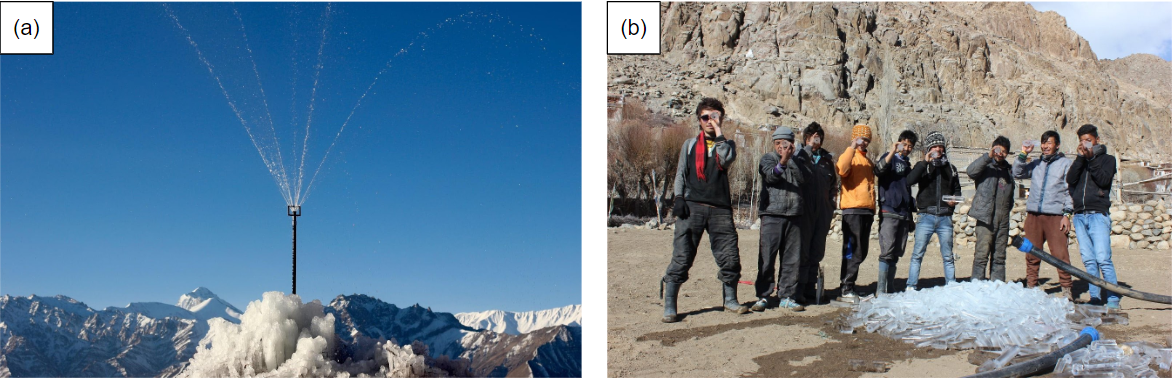
\includegraphics[width=\textwidth]{figs/construction_issues}

  \caption{The present scenario of ice stupa construction is affected by two major issues. (a) Fountains are
  supplied with too much water. (b) Fountain discharge is interrupted frequently due to ice blocks freezing
  inside the pipeline. (Photos: Icestupa Project).}

	\label{fig:issues}
\end{figure}

\textbf{Future scenario}

In the future scenario, the automation system developed in the \textit{Technology} chapter reduces the water
consumption of each ice stupa from $60\,l/min$ to $30\,l/min$. The additional cost to install such a system is
around 1000 USD, which enables two farmers to build eight ice stupas in under 1 week---since there are no pipeline freezing events to deal with (Fig. \ref{fig:icestupa_valley}). The total ice
volumes frozen result in more than twice higher irrigation water supply from mid-April to
mid-June.

\begin{figure}[htb]
	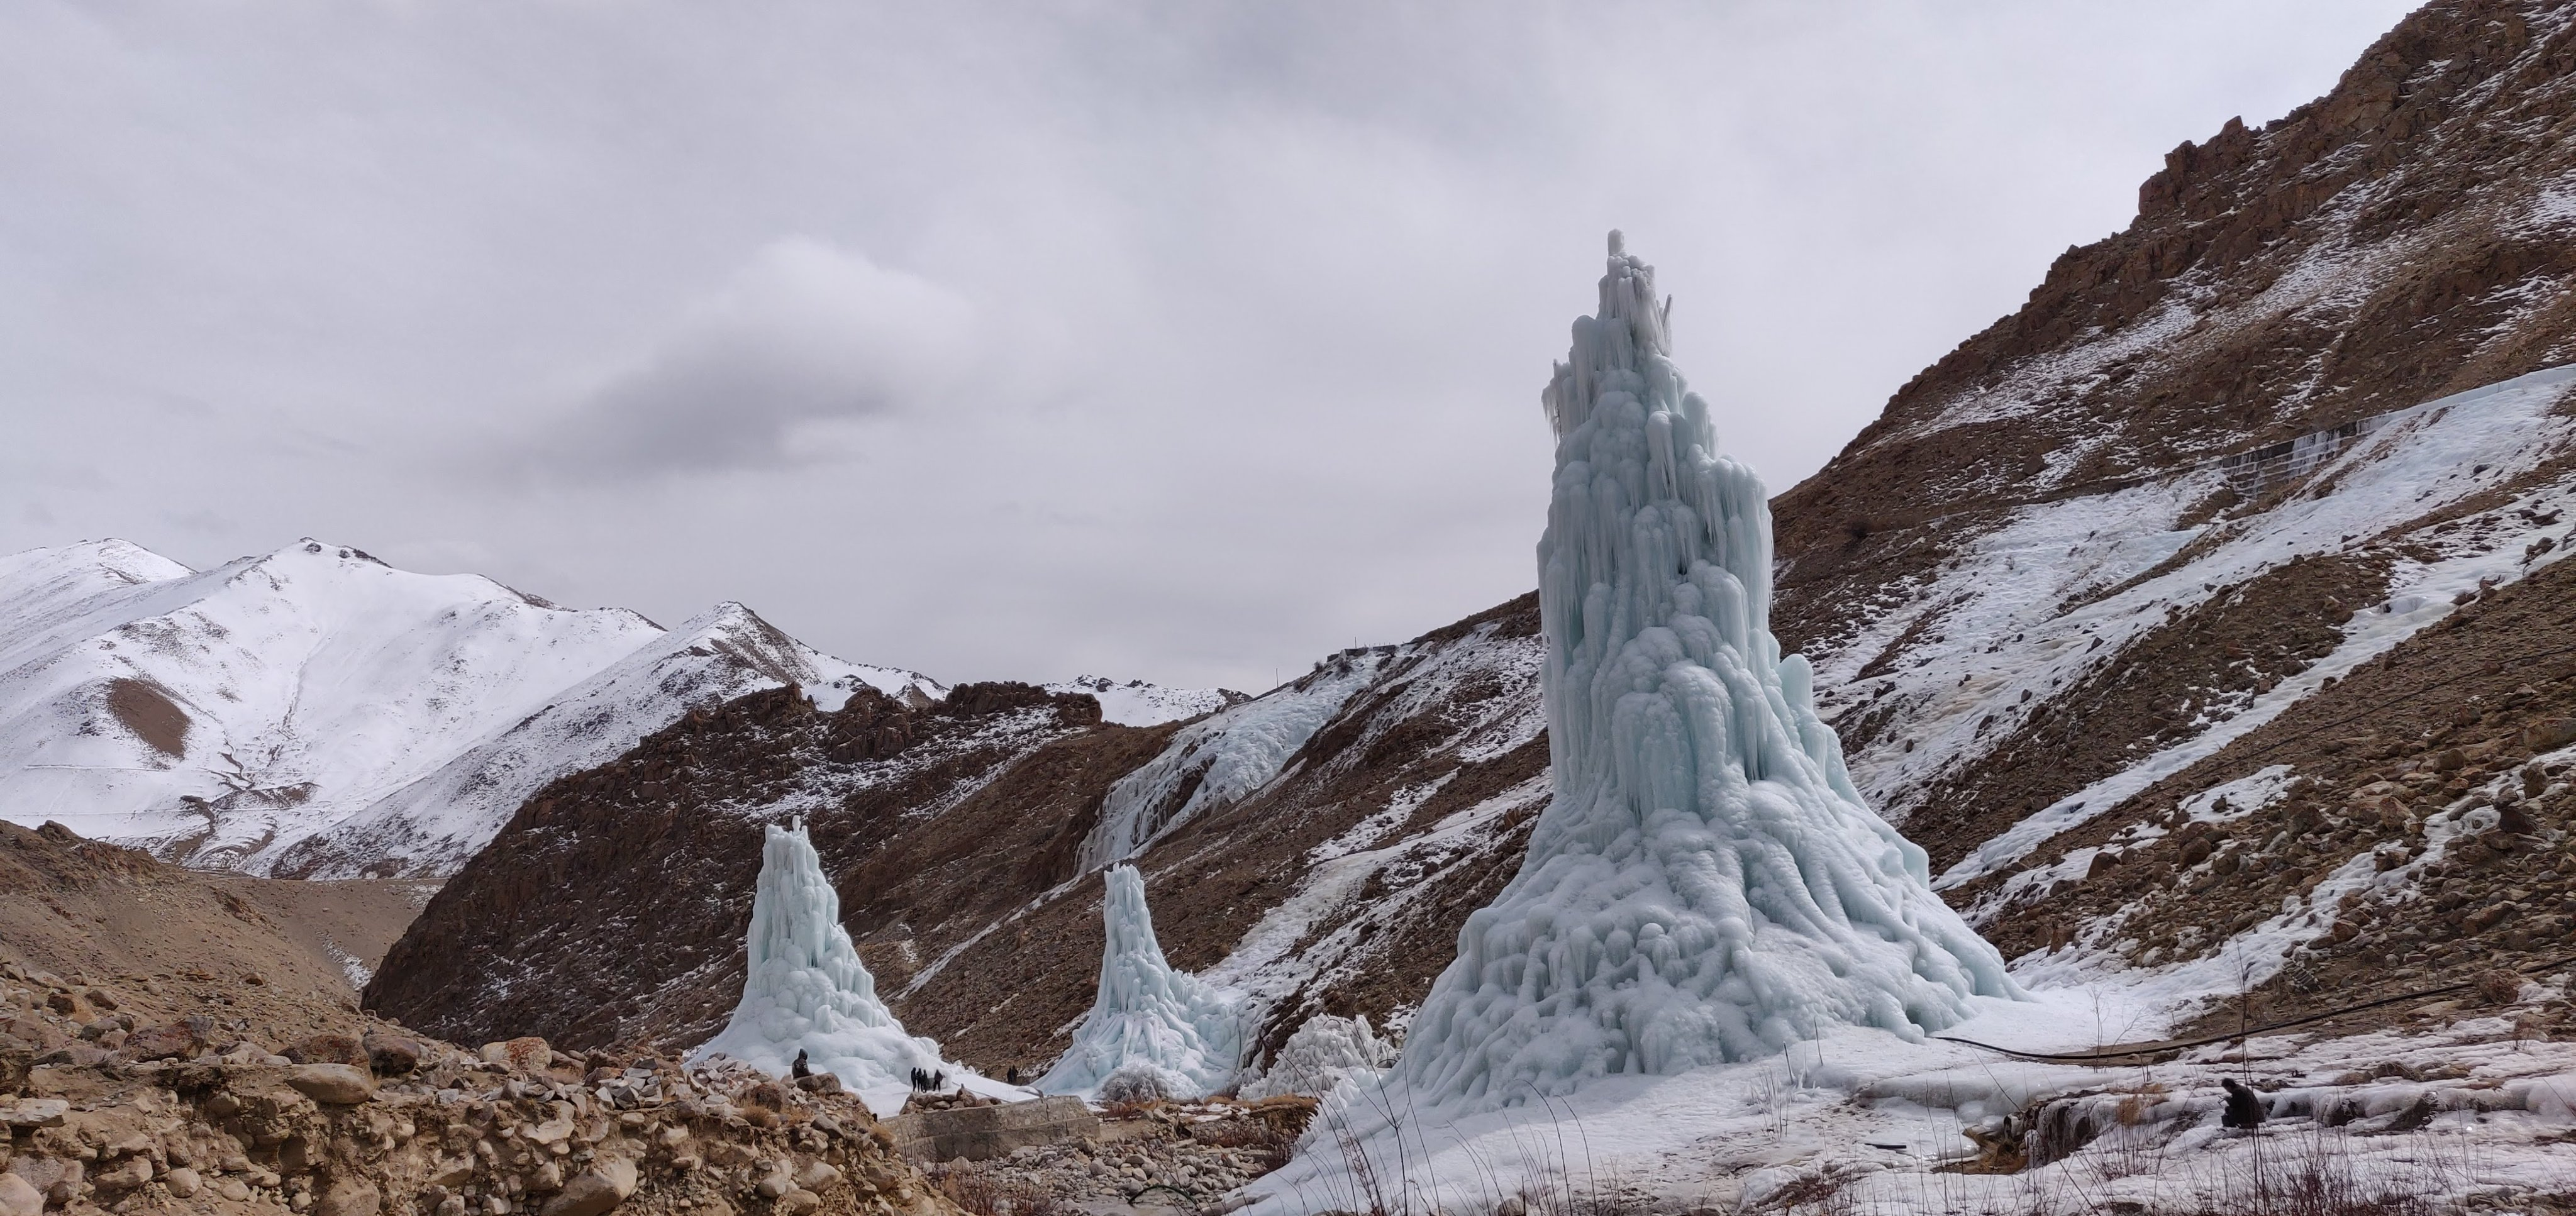
\includegraphics[width=\textwidth]{figs/icestupa_valley}

  \caption{More than a month of effort from a dozen farmers were required to build five ice stupas across the
  Gangles valley in the winter of 2019/20. This research provides tools that two farmers can leverage to
  guarantee twice more winter water storage and reduce maintenance requirements to just a few days. (Photo:
  S. Balasubramanian).}

	\label{fig:icestupa_valley}
\end{figure}

\section{Conclusions}

Glaciers provide an important buffer for highly seasonal precipitation regimes
\citep{kaserContributionPotentialGlaciers2010}. Under the currently available climate change projections, glacial mass loss is expected to continue in future decades, and several smaller glaciers are expected to disappear completely \citep{rabatelCurrentStateGlaciers2013}.

These trends stress the importance of increased water storage capacity for glacierized catchments as a pathway
for climate adaptation. Because of the challenges and costs related to traditional storage efforts, \ac{AIRs} can
be a better tool to adapt to reduced glacial runoff. To quantify their adaptation potential, the volume dynamics of \ac{AIR} melting need to be comprehended, but also how their meltwater contributes to
current and future water use. 

In this thesis, volume variations among eighteen \ac{AIRs} are studied, and their corresponding magnitudes
are explained in terms of the influence of the chosen location's meteorology and topography and the construction
strategy used. Three energy and mass balance models are used to simulate \ac{AIR} evolution using data from field
measurements in Gangles, India and Guttannen, Switzerland. The use of these datasets, in combination with the
models, facilitated an accurate representation of the complex evolution typical of an \ac{AIR}. Although the
approach is demonstrated on specific locations, it can be extended using the open-sourced models and global
reanalysis datasets to account for spatiotemporal meteorological influences of future locations on \ac{AIR}'s
volume dynamics. The main conclusions are summarized below:

\begin{figure}[htb]
  \centering
	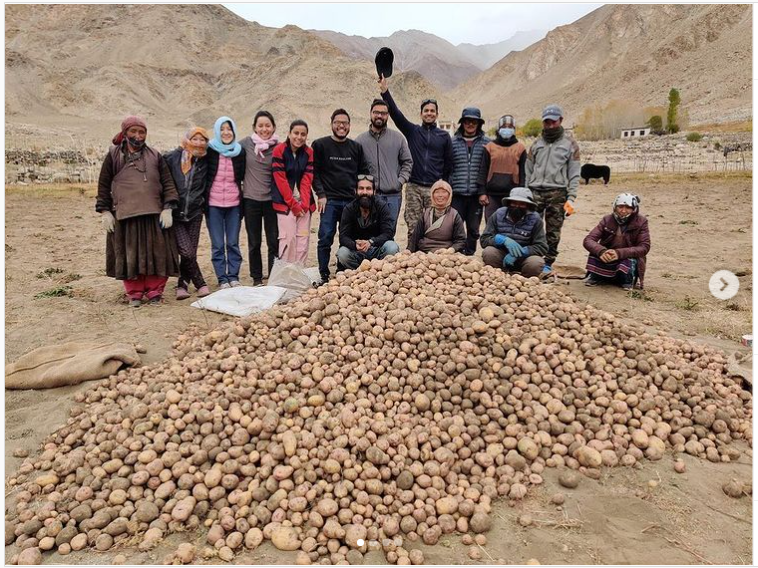
\includegraphics[width=8 cm]{figs/Kullum_potatoes}
	\caption{One of the deserted villages in Ladakh where \ac{AIR} meltwater supported a harvest of 1300 $kg$ of
		potatoes in October, 2021. (Photo: Icestupa Project).}
	\label{fig:kullum_potatoes}
\end{figure}

\begin{enumerate}

  \item The Indian construction site produced long-lasting \ac{AIRs} with four times larger maximum ice volumes
    since it was colder, drier, and less cloudy compared with the Swiss construction site. Thus, the \ac{AIR}
    technology maybe suited to serve as a water management strategy, especially in some dry and cold mountain
    catchments, such as in \ac{HMA} or the Andes.

  \item Water losses of ice stupas were observed to be up to 80\% due to excessive water input. However, the use
    of automated fountain scheduling strategies can lower their water consumption up to 10 times while reducing
    their maintenance requirements.

\end{enumerate}

While the spatiotemporal dynamics of \ac{AIR} melt are documented in this thesis,
major uncertainty remains on how their meltwater contribution propagates through the hydrological system and
compares against the total discharge of mountain catchments. Future research needs to determine which catchments
can benefit most from the supplementary water supply from these ice harvesting technologies and provide tools that
upscale their meltwater supply.

% Model development is an art where subjective choices seek a balance between a model's simplicity
% and its accuracy.
